\documentclass[12pt]{report}
\usepackage[utf8]{inputenc}
\usepackage[russian]{babel}
%\usepackage[14pt]{extsizes}
\usepackage{listings}
\usepackage{graphicx}
\usepackage{amsmath,amsfonts,amssymb,amsthm,mathtools} 
\usepackage{float}

% Для листинга кода:
\lstset{ %
language=C++,                 % выбор языка для подсветки (здесь это С)
basicstyle=\small\sffamily, % размер и начертание шрифта для подсветки кода
numbers=left,               % где поставить нумерацию строк (слева\справа)
numberstyle=\tiny,           % размер шрифта для номеров строк
stepnumber=1,                   % размер шага между двумя номерами строк
numbersep=5pt,                % как далеко отстоят номера строк от подсвечиваемого кода
showspaces=false,            % показывать или нет пробелы специальными отступами
showstringspaces=false,      % показывать или нет пробелы в строках
showtabs=false,             % показывать или нет табуляцию в строках
frame=single,              % рисовать рамку вокруг кода
tabsize=2,                 % размер табуляции по умолчанию равен 2 пробелам
captionpos=t,              % позиция заголовка вверху [t] или внизу [b] 
breaklines=true,           % автоматически переносить строки (да\нет)
breakatwhitespace=false, % переносить строки только если есть пробел
escapeinside={\#*}{*)}   % если нужно добавить комментарии в коде
}

% Для измененных титулов глав:
\usepackage{titlesec, blindtext, color} % подключаем нужные пакеты
\definecolor{gray75}{gray}{0.75} % определяем цвет
\newcommand{\hsp}{\hspace{20pt}} % длина линии в 20pt
% titleformat определяет стиль
\titleformat{\chapter}[hang]{\Huge\bfseries}{\thechapter\hsp\textcolor{gray75}{|}\hsp}{0pt}{\Huge\bfseries}


% plot
\usepackage{pgfplots}
\usepackage{filecontents}
\usetikzlibrary{datavisualization}
\usetikzlibrary{datavisualization.formats.functions}
\begin{filecontents}{LevR.dat}
100 45504
200 344852
300 1626090
400 4410053
500 8809530
600 15523926
700 27314819
800 36896674
900 151438792
1000 253111941
\end{filecontents}

\begin{filecontents}{LevT.dat}
100 50613
200 254889
300 1164803
400 3277843
500 6466829
600 10441740
700 20235150
800 27982176
900 115139281
1000 199701561
\end{filecontents}

\begin{filecontents}{DamLevR.dat}
100 22663
200 189215
300 937882
400 2605948
500 5077237
600 9041331
700 15047492
800 20829956
900 85256627
1000 158414218
\end{filecontents}



\begin{filecontents}{LevR1.dat}
101 45393
201 386372
301 1557256
401 4538718
501 9009942
601 15214595
701 26603522
801 37648086
901 139235577
1001 278285719
\end{filecontents}

\begin{filecontents}{LevT1.dat}
101 35265
201 364594
301 1113414
401 3314034
501 6511456
601 11947585
701 20274021
801 26844301
901 136919210
1001 212082553
\end{filecontents}

\begin{filecontents}{DamLevR1.dat}
101 38152
201 196174
301 919775
401 2652528
501 5171817
601 10328122
701 15001586
801 20867237
901 108043316
1001 165932409
\end{filecontents}



\begin{document}
%\def\chaptername{} % убирает "Глава"
\begin{titlepage}
	\centering
	{\scshape\LARGE МГТУ им. Баумана \par}
	\vspace{3cm}
	{\scshape\Large Лабораторная работа №7\par}
	\vspace{0.5cm}	
	{\scshape\Large По курсу: "Анализ алгоритмов"\par}
	\vspace{1.5cm}
	{\huge\bfseries Поиск подстроки в строке\par}
	\vspace{2cm}
	\Large Работу выполнила: Лаврова Анастасия, ИУ7-55Б\par
	\vspace{0.5cm}
	\LargeПреподаватели:  Волкова Л.Л., Строганов Ю.В.\par

	\vfill
	\large \textit {Москва, 2019} \par
\end{titlepage}

\tableofcontents

\newpage
\chapter*{Введение}
\addcontentsline{toc}{chapter}{Введение}
Целью данной лабораторной работы является изучение алгоритмов поиска подстроки в строке, в частности, алгоритма Кнута-Морриса-Пратта и алгоритма Бойера-Мура.\\
 Задачи лабораторной работы: реализовать алгоритмы Кнута-Морриса-Пратта и Бойера-Мура.


\chapter{Аналитическая часть}
Поиск подстроки в строке — одна из простейших задач поиска информации. Поиск подстроки в строке применяется в виде встроенной функции в текстовых редакторах, СУБД, поисковых машинах, языках программирования и т. п.\\

Пусть дана некоторая строка T (текст) и подстрока W (шаблон). Задача поиска подстроки сводится к поиску вхождения шаблона W в указанной строке T. Строго задача формулируется следующим образом: пусть задан массив T из N элементов и массив W из M элементов, $0 < M \leqslant N$. Если алгоритм поиска подстроки обнаруживает вхождение W в T, то возвращается индекс, указывающий на первое совпадение подстроки со строкой.



\section{Стандартный алгоритм}

Простейшим алгоритмом является примитивный алгоритм. Рассмотрим псевдокод этого алгоритма:\\

\begin{enumerate}
\item[1)] I = 1, J = 1 
\item[2)] Сравнение T[I] с W[J] 
\item[3)] Совпадение: J = J + 1, I = I +1 
\item[4)] Несовпадение: J = 1, I = I + 1 
\item[5)] Если J = M, то подстрока найдена
\item[6)] Если I + M > N, то подстрока отсутствует
\end{enumerate}

\section{Алгоритм Кнута-Морриса-Пратта}

Идея алгоритма заключается в том, что при каждом несовпадении T[I] и W[J] мы сдвигаемся не на единицу, а на J, так как меньшие сдвиги не приведут к полному совпадению. Однако, этот алгоритм поиска дает выигрыш только тогда, когда несовпадению предшествовало некоторое число совпадений, иначе алгоритм аналогичен примитивному. Так как совпадения встречаются реже, чем несовпадения, выигрыш в большинстве случаев незначителен. \\
Алгоритм Кнута-Морриса-Пратта основан на принципе конечного автомата.В этом алгоритме состояния помечаются символами, совпадение с которыми должно в данный момент произойти. Из каждого состояния имеется два перехода: один соответствует успешному сравнению, другой — несовпадению. Успешное сравнение переводит нас в следующий узел автомата, а в случае несовпадения мы попадаемв предыдущий узел, отвечающий образцу. \\

Рассмотрим нахождение в строке "abeccacbadbabbad" подстроки "abbad" и построим следующий автомат (рис 1.1), где состояния маркируются ожидаемыми символами:\\

\begin{figure}[h!]
        	\begin{center}
        		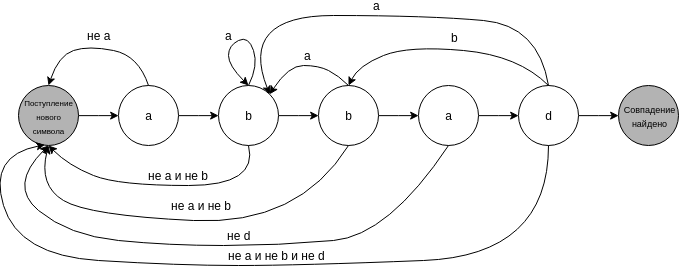
\includegraphics[scale=0.5]{avt_1}
        		\caption{ Конечный автомат в алгоритме Кнута-Морриса-Пратта}
        		\label{fig:def}
        	\end{center}
        \end{figure}


\section{Алгоритм Бойера-Мура}

Алгоритм Бойера-Мура из трех алгоритмов считается наиболее быстрым. В среднем он делает сравнений меньше, чем N. Данный алгоритм считается стандартным для поиска на странице браузера или в текстовых редакторах. \\
Преимущество этого алгоритма в том, что ценой некоторого количества предварительных вычислений над шаблоном (но не над строкой, в которой ведётся поиск) шаблон сравнивается с исходным текстом не во всех позициях — часть проверок пропускаются как заведомо не дающие результата. Идея БМ-поиска – сравнение символов начинается с конца образца, а не с начала, то есть сравнение отдельных символов происходит справа налево. Затем с помощью некоторой эвристической процедуры вычисляется величина сдвига вправо s. И снова производится сравнение символов, начиная с конца образца. 

Рассмотрим нахождение в строке "abeccacbadbabbad" подстроки "abbad" и построим следующий автомат (рис 1.1), где состояния маркируются ожидаемыми символами:\\

\begin{figure}[!h]
        	\begin{center}
        		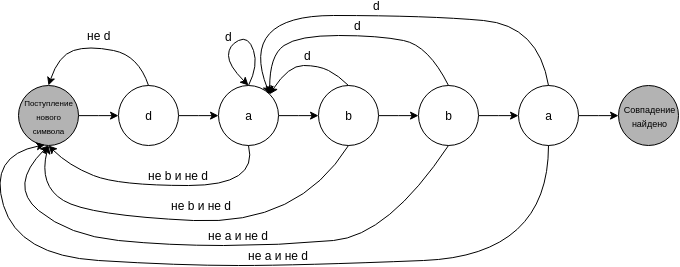
\includegraphics[scale=0.5]{avt_2}
        		\caption{ Конечный автомат в алгоритме Бойера-Мура}
        		\label{fig:def}
        	\end{center}
        \end{figure}





\chapter{Конструкторская часть}
\textbf{Требования к вводу:}\\
Программе на вход подается две строки: текст и шаблон\\
\textbf{Требования к программе:}\\
Программа должна находить первое вхождение шаблона в текст и его индекс (индексация строк начинается с нуля) \\


\section{Разработка реализации алгоритмов}


На рис. 2.1 представлена схема алгоритма Кнута-Морриса-Пратта:\\
На рис. 2.2 представлена схема алгоритма Бойера-Мура:\\

	\begin{figure}[h]
        	\begin{center}
        		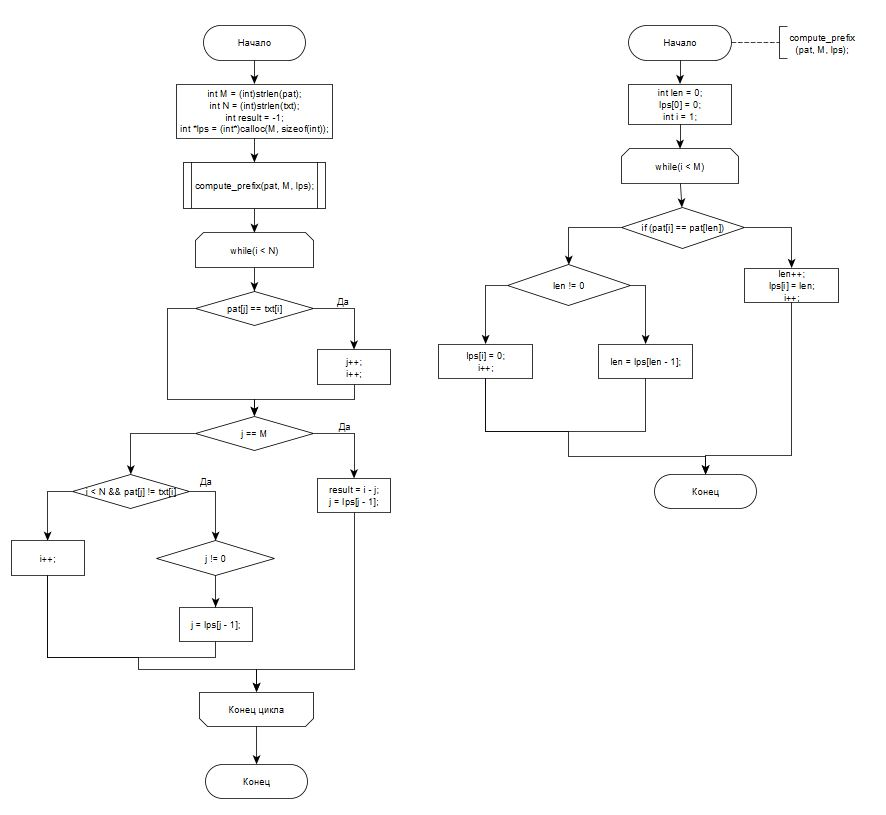
\includegraphics[scale=0.8]{1}
        		\caption{Схема алгоритма Кнута-Морриса-Пратта}
        		\label{fig:def}
        	\end{center}
        \end{figure}


\begin{figure}[h]
        	\begin{center}
        		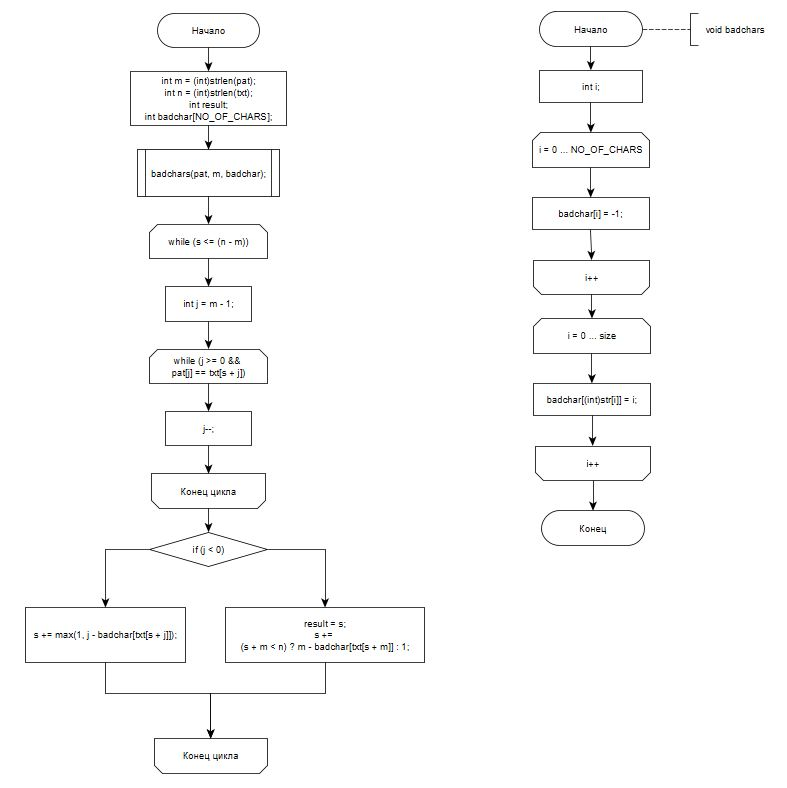
\includegraphics[scale=0.8]{2}
        		\caption{Схема алгоритма Бойера-Мура}
        		\label{fig:def}
        	\end{center}
        \end{figure}


\chapter{Технологическая часть}
\section{Выбор ЯП}
Для реализации программ я выбрала язык программирования C++, так имею большой опыт работы с ним. Среда разработки - Visual Studio. \\

В листинге 3.1 рассмотрен алгоритм Кнута-Морриса-Пратта, а в листинге 3.2 представлен алгоритм Бойера-Мура.\\



\begin{lstlisting}[label=s,caption= Реализация алгоритма Кнута-Морриса-Пратта]
int kmp_search(char* pat, char* txt)
{
	int M = (int)strlen(pat);
	int N = (int)strlen(txt);

	int result = -1;

	int *lps = (int*)calloc(M, sizeof(int));

	compute_prefix(pat, M, lps);

	int i = 0; 
	int j = 0; 
	while (i < N)
	{
		if (pat[j] == txt[i])
		{
			j++;
			i++;
		}

		if (j == M)
		{
			result = i - j;
			j = lps[j - 1];
		}

		else if (i < N && pat[j] != txt[i])
		{
			if (j != 0)
				j = lps[j - 1];
			else
				i++;
		}
	}
	return result;
}

void compute_prefix(char* pat, int M, int* lps)
{
	
	int len = 0;
	lps[0] = 0; 

	int i = 1;
	while (i < M)
	{
		if (pat[i] == pat[len])
		{
			len++;
			lps[i] = len;
			i++;
		}
		else
		{
			if (len != 0)
			{
				len = lps[len - 1];
			}
			else
			{
				lps[i] = 0;
				i++;
			}
		}
	}
}
\end{lstlisting}

	\begin{lstlisting}[label=p,caption=Реализация алгоритма Бойера-Мура]
int bm_search(char *txt, char *pat)
{
	int m = (int)strlen(pat);
	int n = (int)strlen(txt);

	int result;

	int badchar[NO_OF_CHARS];
	
	badchars(pat, m, badchar);

	int s = 0;  
	while (s <= (n - m))
	{
		int j = m - 1;

		while (j >= 0 && pat[j] == txt[s + j])
			j--;

		if (j < 0)
		{
			result = s;

			s += (s + m < n) ? m - badchar[txt[s + m]] : 1;

		}
		else
			s += max(1, j - badchar[txt[s + j]]);
	}

	return result;
}

void badchars(char *str, int size,
	int badchar[NO_OF_CHARS])
{
	int i;

	for (i = 0; i < NO_OF_CHARS; i++)
		badchar[i] = -1;

	for (i = 0; i < size; i++)
		badchar[(int)str[i]] = i;
}
\end{lstlisting}




\chapter{Исследовательская часть}

\section{Тесты}

Далее приведены примеры работы программы (таблица 4.1):\\


\begin{table}[h]
	\caption{Набор тестовых данных}
	%\begin{center}
		\begin{tabular}{| c | c | c |}
	 	\hline
		Текст & Шаблон & Ожидаемый индекс \\ [0.5ex]
	 	\hline\hline
    \grqq there they are \grqq & \grqq they \grqq & 6 \\ \hline
    \grqq there they are \grqq & \grqq there \grqq & 0 \\ \hline
    \grqq there they are \grqq & \grqq are \grqq & 11 \\ \hline
    \grqq there they are \grqq & \grqq there they are \grqq & 0 \\ \hline
	\end{tabular}
%\end{center}
\end{table}
      
      
На рис. 4.1 представлен пример работы программы:\\

	\begin{figure}[h]
        	\begin{center}
        		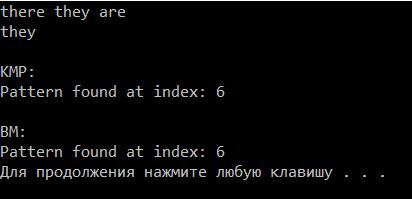
\includegraphics[scale=0.8]{ex1}
        		\caption{Схема алгоритма Кнута-Морриса-Пратта}
        		\label{fig:def}
        	\end{center}
        \end{figure}
	

\section{Пример работы алгоритма Кнута-Морриса-Пратта}

Пусть у нас есть алфавит из пяти символов: a, b, c, d, e и мы хотим найти вхождение образца “abbad” в строке “abeccacbadbabbad”.

Таблица преффиксов будет выглядеть так.

\begin{table}[h]
	%\begin{center}
		\begin{tabular}{| c | c | c | c | c |}
	 	\hline
		a & b & b & a & d \\ \hline
    0 & 0 & 0 & 1 & 0 \\ \hline
		\end{tabular}
	%\end{center}
\end{table}

Начало поиска.

\begin{table}[h]
	%\begin{center}
		\begin{tabular}{| c | c | c | c | c | c | c | c | c | c | c | c | c | c | c | c |}
	 	\hline
		a & b & e & c & c & a & c & b & a & d & b & a & b & b & a & d \\ \hline
    a & b & b & a & d & & & & & & & & & & & \\ \hline
		& & a & b & b & a & d & & & & & & & & & \\ \hline
	  & & & a & b & b & a & d & & & & & & & & \\ \hline
		& & & & a & b & b & a & d & & & & & & & \\ \hline
		& & & & & a & b & b & a & d & & & & & & \\ \hline
		& & & & & & a & b & b & a & d & & & & & \\ \hline
		& & & & & & & a & b & b & a & d & & & & \\ \hline
		& & & & & & & & a & b & b & a & d & & & \\ \hline
		& & & & & & & & & a & b & b & a & d & & \\ \hline
		& & & & & & & & & & a & b & b & a & d & \\ \hline
		& & & & & & & & & & & a & b & b & a & d \\ \hline
		\end{tabular}
	%\end{center}
\end{table}

Совпадение найдено.

\begin{table}[h]
	%\begin{center}
		\begin{tabular}{| c | c | c | c | c | c | c | c | c | c | c | c | c | c | c | c |}
	 	\hline
		a & b & e & c & c & a & c & b & a & d & b & a & b & b & a & d \\ \hline
      &   & a & b & b & a & d & & & & & & & & & \\ \hline
		\end{tabular}
	%\end{center}
\end{table}


\section{Пример работы алгоритма Бойера-Мура}

Пусть у нас есть алфавит из пяти символов: a, b, c, d, e и мы хотим найти вхождение образца “abbad” в строке “abeccacbadbabbad”.

Таблица смещений будет выглядеть так.

\begin{table}[h!]
	%\begin{center}
		\begin{tabular}{| c | c | c | c | c |}
	 	\hline
		a & b & c & d & e \\ \hline
    1 & 2 & 5 & 5 & 5 \\ \hline
		\end{tabular}
	%\end{center}
\end{table}

Начало поиска.

\begin{table}[!h]
	%\begin{center}
		\begin{tabular}{| c | c | c | c | c | c | c | c | c | c | c | c | c | c | c | c |}
	 	\hline
		a & b & e & c &  \textcolor{red}{c} & a & c & b & a & d & b & a & b & b & a & d \\ \hline
    a & b & b & a &  \textcolor{red}{d} & & & & & & & & & & & \\ \hline
		\end{tabular}
	%\end{center}
\end{table}

Последний символ образца не совпадает с наложенным символом строки. Сдвигаем образец вправо на 5 позиций.


\begin{table}[h!]
	%\begin{center}
		\begin{tabular}{| c | c | c | c | c | c | c | c | c | c | c | c | c | c | c | c |}
	 	\hline
		a & b & e & c & c & a & \textcolor{red}{c} & \textcolor{green}{b} & \textcolor{green}{a} & \textcolor{green}{d} & b & a & b & b & a & d \\ \hline
     &  &  &  & & a & \textcolor{red}{b} & \textcolor{green}{b} & \textcolor{green}{a} & \textcolor{green}{d} & & & & & & \\ \hline
		\end{tabular}
	%\end{center}
\end{table}

Второй символ не совпадает, сдвигаем на 5 символов вправо.

\begin{table}[h!]
	%\begin{center}
		\begin{tabular}{| c | c | c | c | c | c | c | c | c | c | c | c | c | c | c | c |}
	 	\hline
		a & b & e & c & c & a & \textcolor{red}{c} & \textcolor{green}{b} & \textcolor{green}{a} & \textcolor{green}{d} & b & a & b & b & \textcolor{red}{a} & d \\ \hline
     &  &  &  &  &  &  &  &  &  & a & b & b & a & \textcolor{red}{d} & \\ \hline
		\end{tabular}
	%\end{center}
\end{table}

Последний символ не совпадает, сдвигаем на один символ вправо.

\begin{table}[h!]
	%\begin{center}
		\begin{tabular}{| c | c | c | c | c | c | c | c | c | c | c | c | c | c | c | c |}
	 	\hline
		a & b & e & c & c & a & c & b & a & d & b & \textcolor{green}{a} & \textcolor{green}{b} & \textcolor{green}{b} & \textcolor{green}{a} & \textcolor{green}{d} \\ \hline
     &  &  &  &  &  &  &  &  &  &  & \textcolor{green}{a} & \textcolor{green}{b} & \textcolor{green}{b} & \textcolor{green}{a} & \textcolor{green}{d} \\ \hline
		\end{tabular}
	%\end{center}
\end{table}

Совпадение найдено.




\section{Вывод}

В данном разделе были приведены примеры работы программы.



\chapter*{Заключение}
\addcontentsline{toc}{chapter}{Заключение}
В ходе выполнения данной лабораторной работы были изучены два алгоритма для поиск подстроки в строке: Кнута-Морриса-Пратта и Бойера-Мура. Во время разработки программного обеспечения были получены практические навыки реализации указанных алгоритмов.




\end{document}